
\chapter{Results}



\todo{Today, I changed the test criterion from the output neuron voltage at time $t$ to a mean over a sample of the last
    $20ms$, network performance improved tremendously. Intuitively makes sense, but in particular it makes NEST networks
    diverge less after peak performance is reached. Are fluctuations in output layer activity increasing during late
    stages of training?}

\todo{it might be worth experimenting with different synaptic delays in NEST in order to evaluate learning performance
    under biologically plausible transmission times. How easy this will \textbf{assumably} be to implement in NEST
    deserves note at this point.}

\todo{talk about the fact that NEST synapses are updated, and SpikeEvents stored to ring buffers to be integrated into
    $u_som$ after the synaptic delay. How much of physiological synaptic delays occurs pre- and postsynaptically in
    pyramidal neurons?}

\section{direct feedback connections to interneurons}\label{sec-electric-syns}

\cite{Vaughn2022,Mancilla2007}




\section{Presentation times with latent equilibrium}

In order to validate the performance of my implementations, I replicated a parameter study from \cite{Haider2021}[Fig.
    3]. The results for the NEST network using spiking neurons with default parameters \todo{elaborate on this} are shown in
Figure \ref{fig-bars-le-snest}. A



\begin{figure}
    \centering
    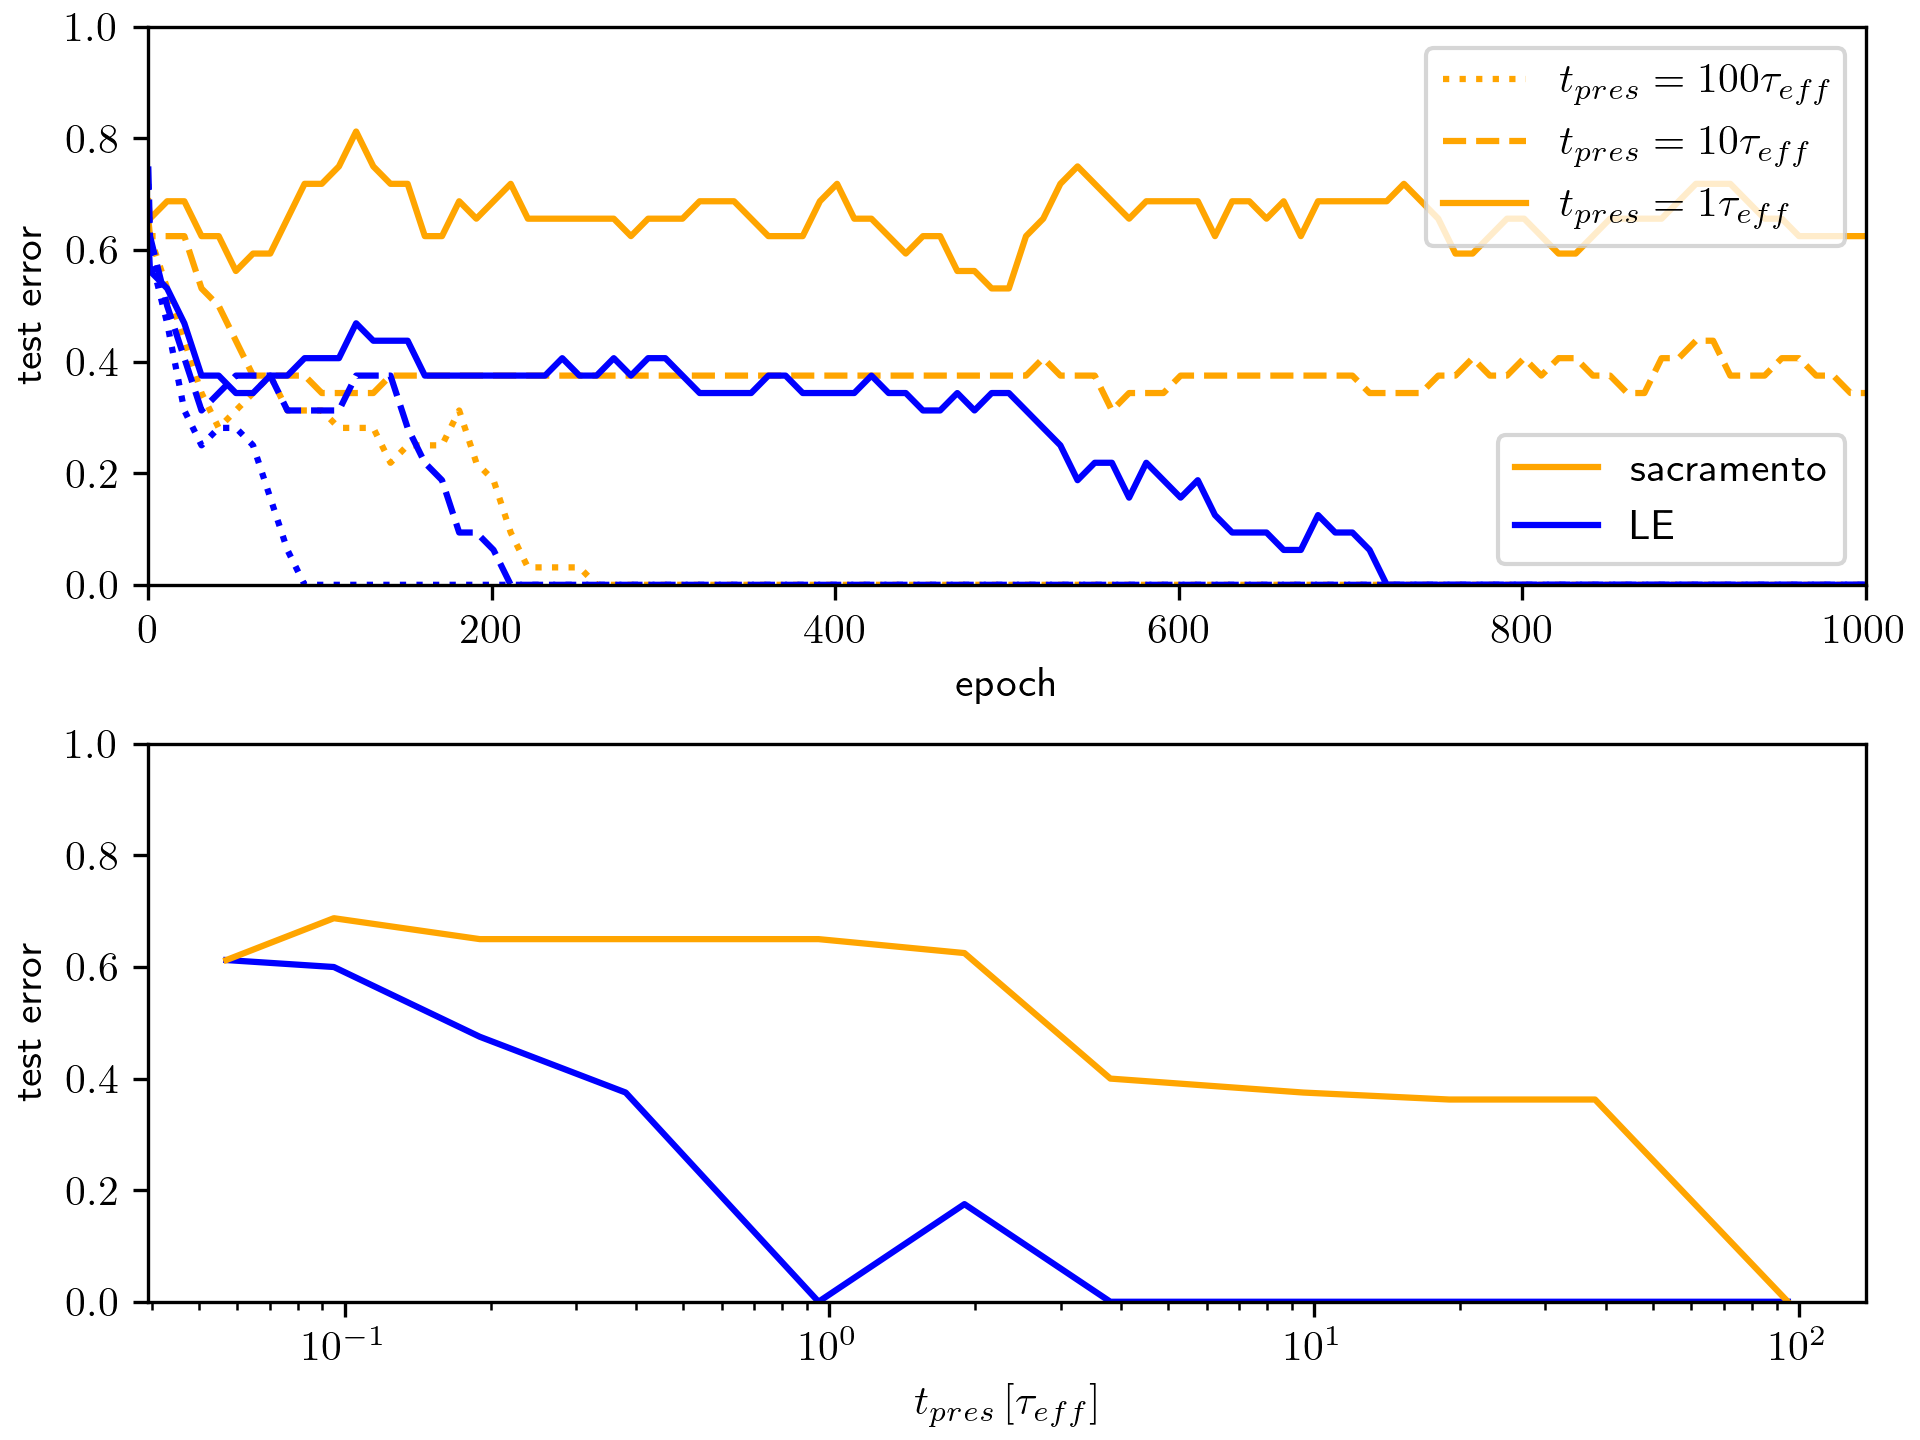
\includegraphics[width=0.9\textwidth]{fig_3_snest}
    \caption{Replication of Figure 3 from \cite{Haider2021} using networks of spiking neurons in the NEST simulator.
        \textbf{A:} Comparison between Original pyramidal microcircuit network by \cite{sacramento2018dendritic} and 
        Latent equilibrium
        variant from \cite{Haider2021}. Shown is the training of a network with 9-30-3 neurons on the 'Bars' Dataset from
        \todo{describe it} with three different stimulus presentation times. \textbf{B:} Test performance after 1000 Epochs as a
        function of stimulus presentation time.}
    \label{fig-bars-le-snest}
\end{figure}

\begin{figure}

\end{figure}




























\chapter{room for random observations}

\begin{itemize}
    \item When reducing the \texttt{weight\_scale} parameter weights converge to lower absolute levels. I.e. mean abs
          weight drops from 0.5 to approx 0.1
    \item When reducing the size of the bar dataset by just 1 element, much simpler networks are capable of learning the
          task at lower t\_pres. Failure to learn shows strange behaviour: the network fails to predict any sample of
          one group, with the group which it fails to represent switching every now and then.
    \item increasing apical $C_m$ for spiking neurons was a straight banger.
    \item I switched input neurons for poisson\_generators. This is faster, but will fuck up any simulations that rely
          on precise spike timing, since the generator redraws spikes for every target nrn.
\end{itemize}